\documentclass[tikz,border=5pt]{standalone}
\usepackage{fontspec}
\setmainfont{Times New Roman}
\usepackage{unicode-math}
\setmathfont{Cambria Math}
\usetikzlibrary{shapes.geometric,shapes.misc,positioning,fit,backgrounds,arrows.meta,calc}

\begin{document}
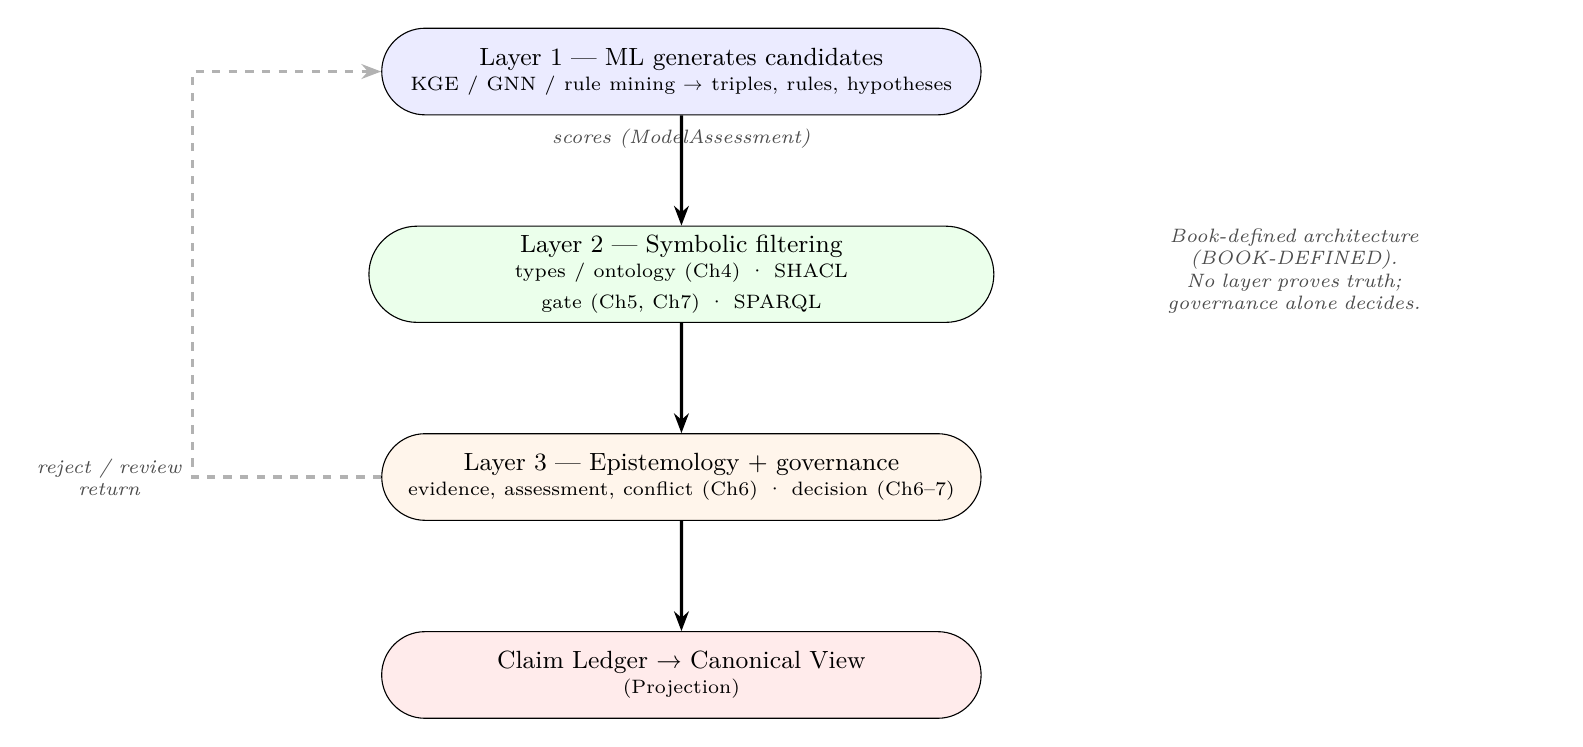
\begin{tikzpicture}[
  stage/.style={rounded rectangle, draw, align=center, minimum width=5.2cm, minimum height=1.1cm, font=\small},
  arrow/.style={-{Stealth[length=2.5mm]}, very thick},
  label/.style={font=\scriptsize\itshape, text=gray!60!black},
]

% === Layer 1: ML candidates ===
\node[stage, fill=blue!8, text width=7.2cm] (ml) at (0, 3.8)
  {Layer 1 — ML generates candidates\\[-2pt]\scriptsize KGE / GNN / rule mining $\rightarrow$ triples, rules, hypotheses};
\node[label, below=0.05cm of ml.south] {scores (ModelAssessment)};

% === Layer 2: symbolic filter ===
\node[stage, fill=green!8, text width=7.2cm, below=1.4cm of ml]
  (sym) {Layer 2 — Symbolic filtering\\[-2pt]\scriptsize types / ontology (Ch4) · SHACL gate (Ch5, Ch7) · SPARQL};

% === Layer 3: epistemic + governance ===
\node[stage, fill=orange!8, text width=7.2cm, below=1.4cm of sym]
  (epi) {Layer 3 — Epistemology + governance\\[-2pt]\scriptsize evidence, assessment, conflict (Ch6) · decision (Ch6–7)};

% === Ledger ===
\node[stage, fill=red!8, text width=7.2cm, below=1.4cm of epi]
  (ledger) {Claim Ledger → Canonical View\\[-2pt]\scriptsize (Projection)};

\draw[arrow] (ml) -- (sym);
\draw[arrow] (sym) -- (epi);
\draw[arrow] (epi) -- (ledger);

% === Feedback: rejected / review back to ML ===
\draw[arrow, dashed, gray!60] (epi.west) -- ++(-2.4,0) node[label, left, align=center] {reject / review\\return} |- (ml.west);

% === Annotation ===
\node[label, align=center, text width=6.4cm, right=1.1cm of sym.south east, anchor=south west]
  {Book-defined architecture\\ (BOOK-DEFINED).\\ No layer proves truth;\\ governance alone decides.};

\end{tikzpicture}
\end{document}